\chapter{Introduction}
\label{chap:introduction}
Chess has been paradigmatic of the discrete deterministic tradition in AI. 
With the rise of the probabilistic and machine learning approaches, the board 
evaluation process has been modulated with probabilistic models 
\cite{baxter1999tdleaf, baxter1999knightcap}, but the 
underlying deterministic search-driven playing mechanism has not changed in the 
last seven decades since the birth of AI. The basic paradigm for chess-playing 
machines  has been to essentially 
generate large search trees by expanding a large set of possible moves upto 
a certain ply-depth heuristically pruning certain nodes, evaluate the leafs 
and select the best move by minimax algorithm. With the exponential advances in 
chip speeds and capacities, this brute force way of computers playing chess 
eventually led Deep Blue to beat Garry Kasparov who was then the reigning world 
champion \cite{campbell2002deep}.\\

Meanwhile the study of machine learning has become popular 
amongst the community focusing on other interesting problems related to three 
major learning paradigms-- supervised learning, unsupervised learning and 
reinforcement learning. However in case of chess, machine learning has 
seldom been used except addressing several disjoint issues, for instance 
learning evaluation weights of various handcrafted features like piece 
values\cite{beal1997learning}, piece-square values\cite{beal1999learning} and 
mobility, while others use machine learning techniques to learn 
opening book moves specifically \cite{hyatt1999book}. Another class of systems 
use co-evolution, where the system learns by 
playing itself 
\cite{vazquez-coello-12_evolutionary_hooke-jeeves-algo_chess-evaluation}  and 
optimizing the parameters 
\cite{bovskovic-brest-11_tuning-chess-evaluation-w-differential-evolution} 
often using evolutionary methods.\\

Recently, deep learning has been rapidly expanding into new domains as a field 
of machine learning. The primary advantage of deep learning systems is the 
ability to learn hierarchical feature representations that make the models 
generalize better to unseen data (explained in greater detail 
in~\ref{subsection:representation}, example in 
figure~\ref{figure:deepmind-fc}). While deep learning methods inspire most of 
the state of the art in image and language categorization tasks 
\cite{krizhevsky2012imagenet,tompson2014efficient,taigman2014deepface,
ciresan2012multi}, there is a lack applications to these discrete search 
situations. Recently, an important achievement of deep learning architectures 
has been in achieving human-like control for the task of playing video games 
through a deep reinforcement learning architecture \cite{deepmind_nips}. The 
prime contribution of the work was the ability to learn human-like control 
directly from high-dimensional sensory input of the video 
games.\label{discussion:deepmind}
\begin{figure}[h]
 \centering
% \vspace*{-0.3in}
%  \hspace*{-1.2in}
 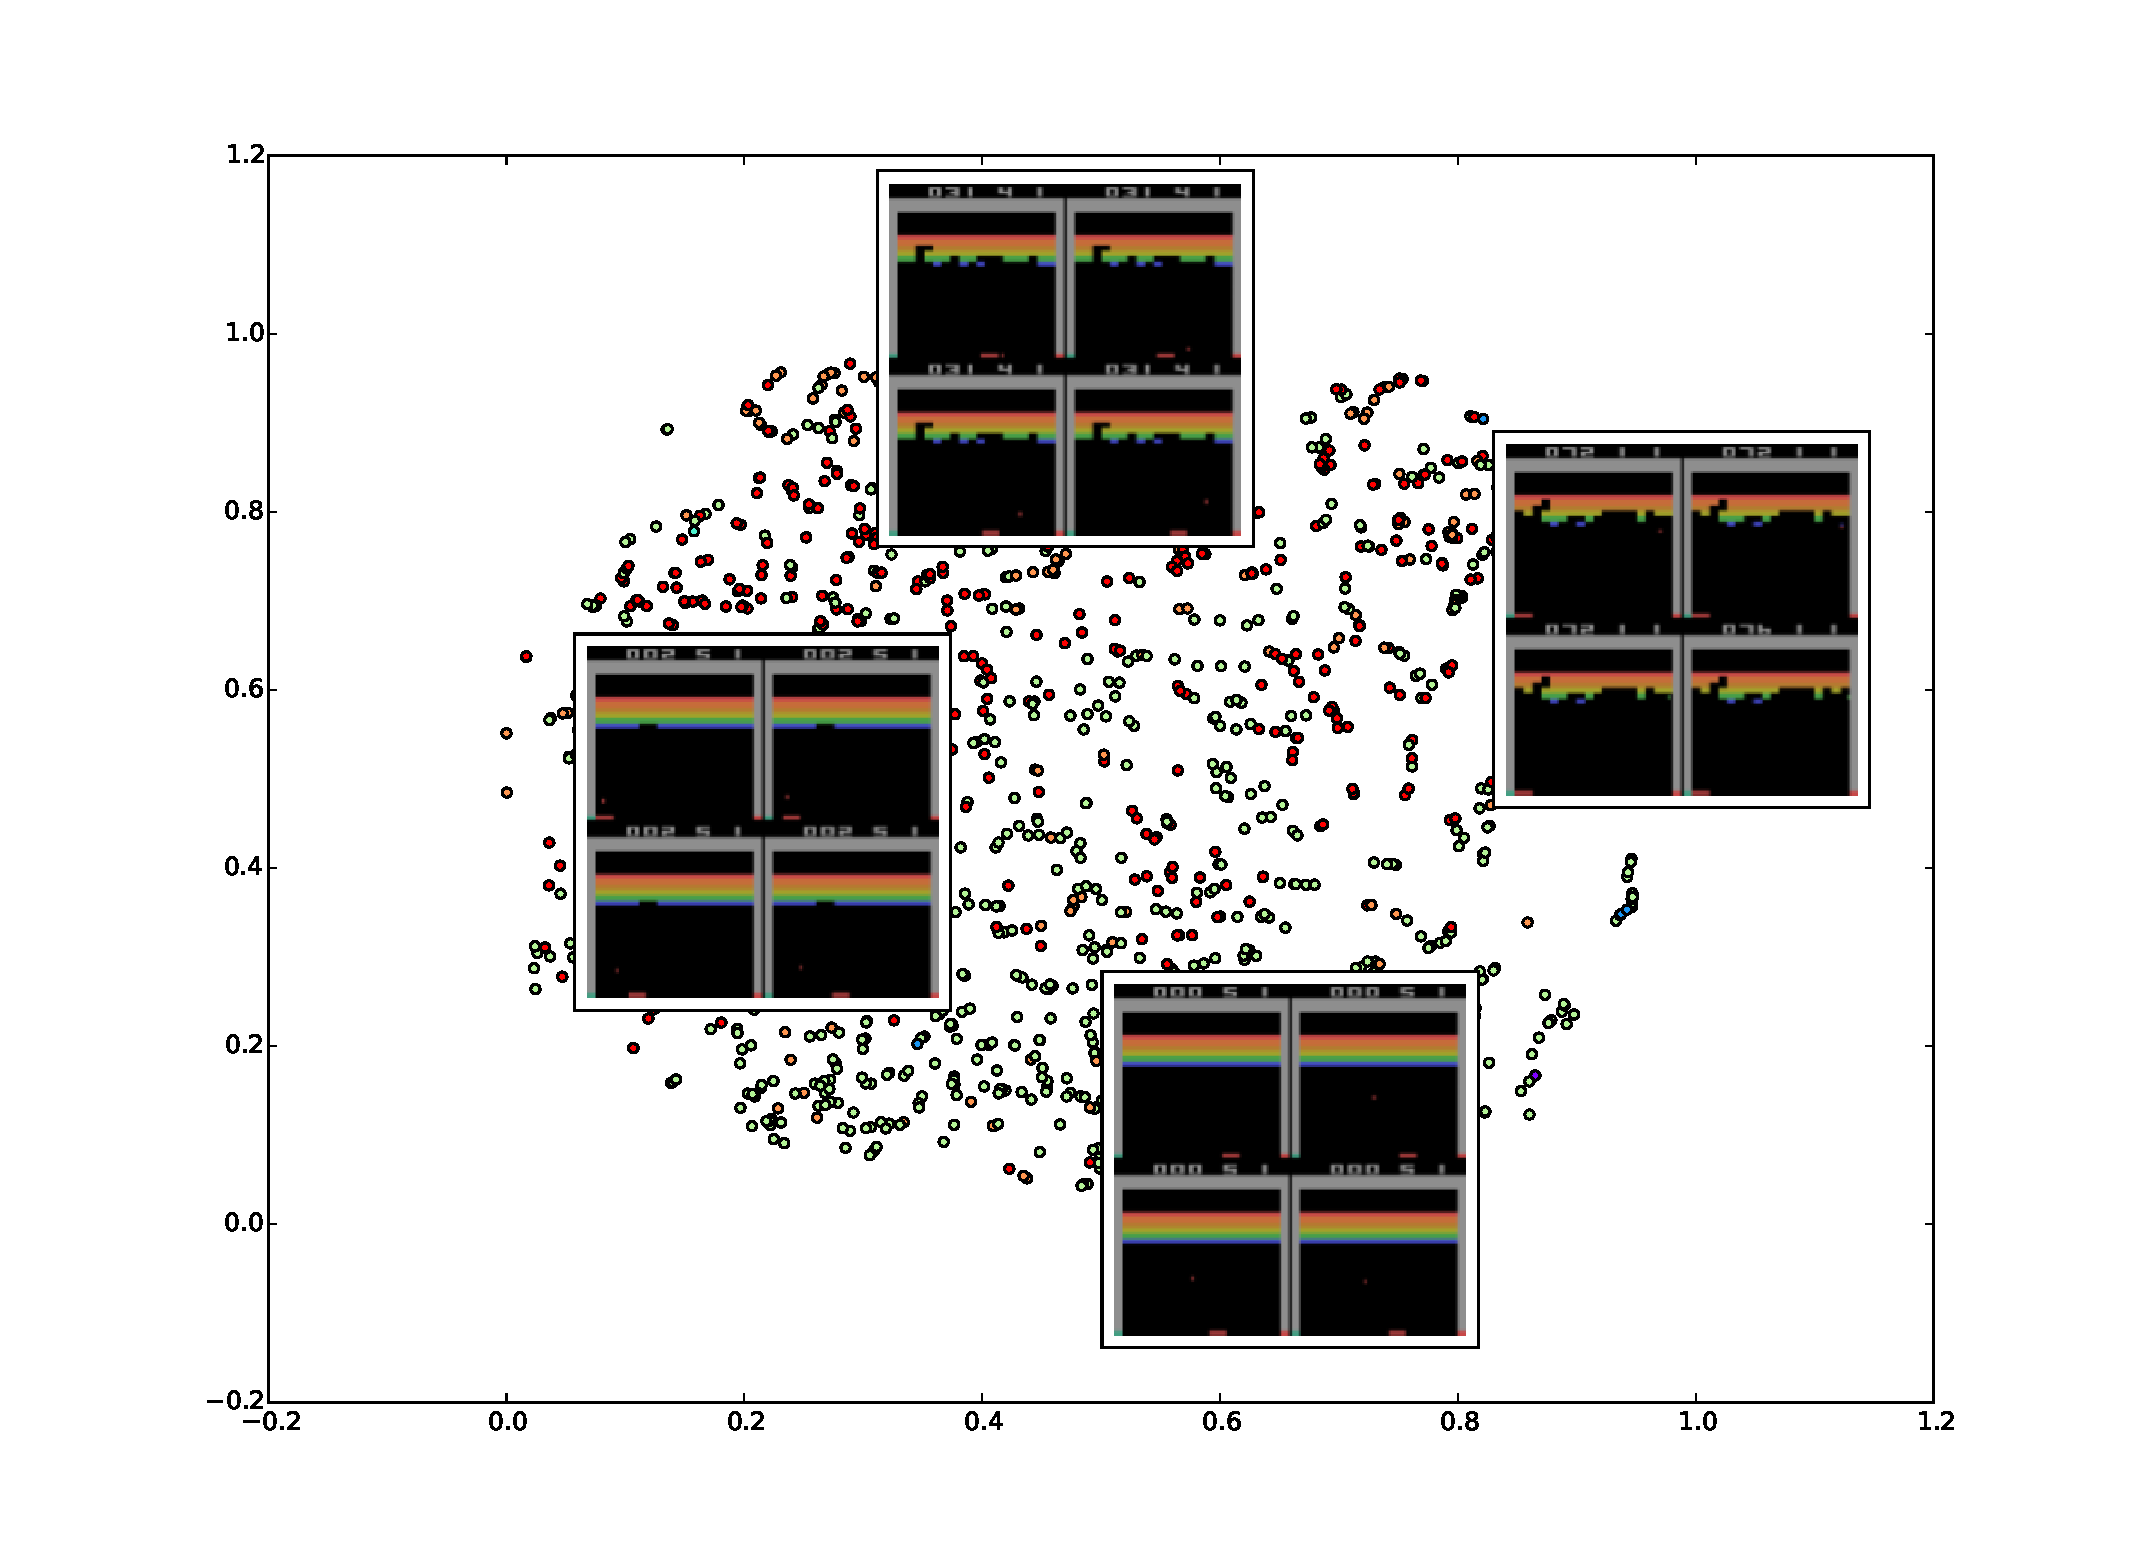
\includegraphics[width=1.1\textwidth, 
scale=0.8]{plots/tsne_breakout_new3_big.pdf}
 
 \caption[Fully connected layer's TSNE embedding in Deepmind's network]{The 
plot shows the TSNE embedding of the last fully connected layer in a network 
trained for the game of Breakout. The two primary colors--green and brown, 
respectively, show the two primary actions learned while playing the game of 
Breakout i.e. left and right respectively and the separation is almost 
apparent. }
\label{figure:deepmind-fc}
\end{figure}
Figure~\ref{figure:deepmind-fc} shows the last fully connected 
layer of a CNN trained to play Breakout trained using a reinforcement learning 
architecture. The separation between the state embeddings which are mapped to 
different actions is visible.\\

However, the deep reinforcement learning architecture in the work of 
\citet{deepmind_nips} performs poorly in deciding the optimal moves for games 
like Pacman etc. where the actions are best decided using a search or planning 
based method. Recently, an extension of this work by \citet*{guo2014deep} 
improved the results by a bit on some games that required extensive 
planning. Using a Monte-Carlo tree search based player to simulate trajectories, 
they trained a CNN based regression model on the generated state-action-value 
instances.\\

This integration of the CNN based RL agent and a planning 
agent having expert control motivates our case of modeling the complex dynamics 
of chess.

\section{Learning chess from scratch}
In this work, we undertake the task of learning to play the game of chess with 
minimal prior knowledge. The capability to learn chess, for our task, can be 
accomplished if a machine can:
\begin{itemize}
 \item Learn to play legal moves
 \item Rank the possible moves without any explicit guidance on relative
    importance of material or position. 
 \item Evaluate board positions
\end{itemize}

To accomplish this task using minimal knowledge prior, we use Convolutional 
neural networks to learn the game directly from board positions, moves and 
outcomes. We will finally evaluate our system on its ability to avoid illegal 
moves, predict good moves at certain board positions and play against a 
traditional search based chess player.\\

We believe that although such a system may not be able to play a championship 
level game, but it can prove to be an example of a chess player that has 
learned from scratch only observing chess games and having no clue of the 
rules.


\section{Aspects of expert human chess playing}
In this section, we look at what motivates us to solve the problem of chess playing as a 
pattern recognition task as opposed to the conventional approaches of 
accomplishing it as a predominantly search problem. We discuss various 
studies which suggest that most of the chess computer AIs that compete with the 
best human chess players don't probably play it the actual way humans do. 
Specifically, we motivate the task of playing chess in a more human way using a 
pattern recognition system in section~\ref{section:chess-as-pr}.\\

Adriaan de Groot, a Dutch chess master and a psychologist, after a deep 
statistical and interpretative analysis of chess players' transcripts of verbal 
utterances, their eye gaze movement and interviewing a number of beginner and 
master level chess players concluded that all players usually examine 40-50 
positions before playing a move. The difference however 
is that the master level players develop pattern recognition skills from 
experience which helps them examine only a few lines of play in much greater 
depth while ignoring the poor moves, where the beginners spend a lot of their 
time \cite{de1996perception}. Another evidence of why this is how humans 
play chess is that humans, especially at the master level, are capable of 
recognizing familiar arrangements of board or specific sets of pieces 
from experiences, rather than random arrangements of the same pieces  
\cite{chase1973perception}. Also unique to humans is the capability to learn 
from experience. This learning can both be ability to recognize patterns from 
the past games or it could be the ability to learn the weaknesses of the 
opponent or learn from his/her own strategic mistakes made.

\subsection{How to become an expert?}
\citet{ericsson2007making}, based on scientific research that 
looked at extraordinary and exceptional performance in a number of fields, 
observes that ``experts are always made, never born''. The author studied 
expertise in 
wide variety of domains ranging from chess to cooking, before concluding that 
the amount and quality of practice were the key factors in the level of 
performance achieved. The author also claims that a minimum of ten years of 
intense training is required before even the most gifted talents can 
win international competitions \cite{ericsson2006cambridge}. An aspect of this 
intense training and practice is that it is deliberate, meaning it 
consists of considerable and sustained efforts to do something which you can't 
already do well. The same goes for chess. Grandmasters, while they are very 
young, have played a huge number of games and also analyze the games they lost 
to eliminate all weaknesses in their gameplay.\\

Before Garry Kasparov, the then reigning world champion, was defeated by Deep 
Blue \cite{campbell2002deep} in May of 1997 in a chess match under tournament 
conditions, the two had a match in February 1996, when Kasparov came from 0-1 
down to win the match 4-2. The reason Kasparov could make a comeback was that 
he learned from Deep Blue's weaknesses and took advantage of them, while the 
deep blue computer responded similarly the next time too. This goes on to tell 
us the difference between a chess computer with no learning capability and a 
human grandmaster who learns about the weaknesses of the opponents. However, 
eventually Deep Blue was destined to beat Kasparov next year, but that was not 
an achieved because of a learning component, but more efficient and deeper 
search along with human intervention for tweaking the computer \cite{cnn-news}. 

\subsection{How are Grandmasters different?}
We associate the ability to play a good game of chess with someone's mental
ability-- such is the intellectual aura about chess. But 
\citet*{bilalic-mcleod-07_does-chess-need-intelligence_young-chess-players} 
suggests that better chess players do not necessarily perform exceptionally 
well in IQ tests. Further, neither are the chess grandmasters known to evaluate 
moves more rapidly then others \cite{de1996perception}. The aspects that mark 
chess grandmasters from others, appear to be similar to markers of expertise 
across a wide range of domains:
\begin{itemize}
 \item The mental representation is in terms of larger chunks, so that
	positions, and possible actions, are encoded more efficiently
	\cite{chase1973perception, gobet-clarkson-04memory_chunks}. In fact, 
the work by \citet*{deepmind_nips} shows that the representation learned by 
deep reinforcement learning architectures (shown in \ref{figure:deepmind-fc}) 
is arranged similarly i.e. states with similar actions are arranged in 
what may be called chunks.
\item Although a grandmaster may evaluate approximately the same number of
	moves as other players, the moves explored by the
	grandmaster are the stronger moves. Thus, presented with a board
	that may arise in a real chess game, the chess expert ``sees'' only a 
few good moves. This is also a type of pattern matching, but the 
complexity is mind-boggling. Perhaps this is possible 
only because the input space is no longer the set of distinct boards, but the 
space of all configurations of chunks, which is much smaller.
\end{itemize}


% \citet{gherrity1993game} introduced the notion of a general learning system, 
% known as the \textit{Search and Learning} system (SAL), that could learn to 
% play any rectangular board based two-player board game with a fixed types of 
% pieces. SAL, trained using temporal difference learning, learns from the 
% outcome of each game it plays. It was tested on Tic-tac-toe, Connect-4 and 
% Chess. It could successfully play Tic-tac-toe and Connect-4, but the level of 
% play he could achieve with a depth of search as 2 in chess was very poor. 
% However, this inspired works like Neurochess \cite{thrun1995learning} which used 
% chess game databases to learn the evaluation function while playing using a 
% standard search-based algorithm.

\subsection{Chess Reasoning as Pattern Recognition}
\label{section:chess-as-pr}
As we discussed above, the master level human chess players are known to 
recognize specific arrangements of the board or a specific set of pieces on the 
board and hence ignore certain poor positions to utilize their time to explore 
more important lines of play in a greater depth. We believe that an expert 
pattern recognition system, such as a human, would be able to recognize these 
patterns learned through experience and hence make a more informed decision to 
play a certain move. In other words, we think that a pattern recognition system 
that has seen enough examples of board positions and the corresponding expert 
moves should be able to predict favorable moves. But at the same time, we expect 
it to remain a necessity to explore those moves upto a greater depth.

% \section{Problem statement}
% In our work, we will take inspiration from these studies seeking a more human 
% way of playing the game of chess rather than computer chess 
% programs that predominantly employ search to make a move, which is a part of 
% what humans do before making a move. In fact, we try to solve a tougher 
% problem than just making a computer play chess well. We want the computer, 
% which has seen enough number of games, to figure out the rules of the game 
% without being explicitly programmed to know the rules of the game. By this 
% task, we also try to account for the generalization capabilities of a human 
% brain by looking at only a few examples of even a very vast set. For this task, 
% we make use of Convolutional neural networks which is a specific artificial 
% neural network architecture inspired by biological vision characteristically 
% suited for pattern recognition tasks (described in greater detail 
% in~\ref{subsection:cnn-background}). We want to emphasize that the our major 
% motivation is not to build a system that can beat other state of the art 
% systems, but to present a proof of concept that chess computers that are 
% inspired by human thinking and pattern recognition, as observed in the 
% case of grandmasters, can also yield a performance comparable to chess 
% programs that are predominantly based on search.


\section{Related work}
In the upcoming text, we will look at some of the related works in the 
fields of learning games using machine learning rather than logic and search. 
Some of the very recent works in combining deep learning with 
reinforcement learning has resulted in human level control of arcade 
games (discussed above). Many of these works have 
inspired us to take up Chess playing as machine learning and pattern recognition 
task. \\

\label{subsection:previous-works}
\subsection{Convolutional Neural Networks for playing Go}
Following the work of \citet{sutskever2008mimicking} which achieved modest 
success due to relatively small sized architecture, \citet{maddison2014move} 
used deep convolutional neural networks to play Go. The network could predict 
the correct move 55\% of the time and beat the traditional search program 
GnuGo in 97\% of the games without using any search and match the performance 
of a state-of-the-art Monte-Carlo tree search that simulates a million 
positions per move. They represent the current board position as a 3 channel 
image, along with adding channels for number of liberties before and after 
move, legality and the rank of the player. Much of the formulation of our 
model is motivated by this representation.\\

\subsection{Go versus Chess}
Using Convolutional networks to predict moves in Go proves to be a great step 
in the direction of building state of the art Go systems. This motivates us to 
use the same technique in predicting moves in the game of Chess. However, we 
must realize that the two games are fundamentally different in many aspects 
that make Go an easier game to play using a Convolutional Network. The game of 
Go has smoother arrangements of positions that are almost continuous 
within and between games.\\

Every move in Go adds a single piece to the board. 
Numerically speaking, making a move in Go using a random draw has a chance of 
$\frac{1}{361}$ on a $19\times 19$ board, while making a move drawing 
randomly the from and to positions in chess is correct with a 
chance of a mere $\frac{1}{4096}$. Also, a single move on a chess board makes a 
change of at least 2 pixels (more than 2 for a piece capture) which is 
significant for an $8\times 8$ board, while in Go only 1 pixel is added to the 
board every move making the transition much smoother than chess. Since, much 
of the knowledge of chess is characterized by strong domain knowledge in a 
logical form, such as ``if bishop on the central diagonal'', ``if the king has 
liberty more than 1'' etc., makes it less intuitive if as compared to the case 
of Go, Convolutional Neural networks can actually model the rules, leave 
aside the optimality of the moves.\\

\subsection{Deep learning for Chess}
This work also inspired a modest attempt of using convolutional neural networks 
to play chess, which achieved minimal success because of a much small dataset 
and weak representation \cite{oshripredicting}. We also acknowledge this work 
to have inspired us to make use of Convolutional neural networks to play chess. 
Other works that use deep learning to play chess do not learn the piece 
arrangements and their relative importances to score the table or evaluate it, 
rather they utilize a set of handcrafted features like king's safety, king's 
liberty, number of rooks on seventh rank etc. \cite{mannen2003learning, 
thrun1995learning} 

\subsection{Learning from Mistakes}
\label{subsection:mistakes-learn}
An important part of playing chess is to remember the each position in which 
the program made a mistake, so that the mistake is not repeated next time the 
position is encountered. The game playing system 
by \citet{epstein-01_learning-to-play-expertly-tutorial-on-hoyle} named HOYLE 
looks at the last position where the losing player could have made an alternate 
move by exhaustively searching the game tree. If the search succeeds, the 
alternate move is recorded and the state is marked as ``significant''. If the 
search fails to find an alternate path to winning position, the state is marked 
as ``dangerous''. In~\ref{subsection:representation-discussion-cnn}, we will 
look at how machine learning architectures like convolutional neural networks 
can provide more generalized representations, so that such ``significant'' and 
``dangerous'' states as well as other similar states are represented and 
searched for efficiently.

\section{Background}
\label{chap:background}
In this section, we will first look at what it means to play the game 
of chess perfectly, before moving on to studying how computers are programmed 
to play 
chess efficiently and exceptionally well. Further we look at some background 
about reinforcement learning, deep learning and 
learning representations and how 
convolutional neural networks, a specific case of deep learning architectures, 
has shaped the field of artificial intelligence especially in the area of 
pattern recognition.% in~\ref{subsection:cnn-background}. 
% In section~\ref{subsection:previous-works}, we also introduce some effective 
% approaches that solve problems similar to the task at hand like playing Atari 
% games using deep reinforcement learning, predicting moves in the games of Go 
and 
% evaluating moves in chess.  
\subsection{Ideal Leaf-evaluation function}
\label{section:solving}
Solving chess refers to finding an optimal strategy for playing chess. Chess 
has 
a finite number of states, estimated to be around $10^{43}$ 
by \citet{shannon1950xxii}. \citet{zermelo1913anwendung} proved that a 
hypothetically determinable optimal strategy does exist for chess.\\
In a weaker sense, each position can be assigned as a win for white, a win for 
Black or a forced draw if both the players are using the optimal strategy. We 
can formulate this as a function $f$ for each board position using the 
procedure 
below.
\begin{enumerate}
\item Assign all the positions with no further play possible as:
\[f(position) = \begin{cases}
1 \text{ , if White has won}\\
0 \text{ , if it is a draw}\\
-1 \text{ , if Black has won}
\end{cases}\]
\item Use the recursive rule up the game tree:
\[f(p) = \max\limits_{p\rightarrow p'} (-f(p'))\]
where $p'$ is a position reachable in one move from position $p$.\\
Here the negative sign means that a win for the opponent is a loss for the 
player in consideration and vice-versa.
\end{enumerate} 
The above recursive rule is the same as the minimax algorithm for the case when 
the game tree for chess is fully grown. The function $f$ gives us the 
``perfect'' evaluation function to play a chess game. While playing the game, 
we 
just need to choose the move which takes us to the board position $p$ for which 
$f(p)=1$.\\

But this evaluation function, $f$, cannot be computed with the computing 
resources available as of now. Hence, we need to resort to approximations of 
$f(p)$.


\subsection{Playing Chess using Computers}
\label{section:playing-background}
The first study on computers playing the game of chess was done by 
\citet{shannon1950xxii}. He predicted two main search strategies that would 
evolve with computers being programmed to play chess--
\begin{enumerate}
\item ``Type A" programs would use a ``brute force" examination of all the 
board 
positions possible through valid moves upto a certain depth of play.
\item ``Type B" programs would employ a ``quiescence search" looking at only a 
few good moves for each position. 
\end{enumerate}
He also predicted the ``Type A" programs to be impractical because of the 
massive search space. For even a computer evaluating $10^6$ moves per second, a 
lookahead of 3 moves for both sides, when an average of 30 moves are available 
for each board position, the program would take around 13 minutes.\\
\begin{table}[h]
\centering
%\resizebox{\textwidth}{!}
\caption{Time taken to explore 30 moves per position at $10^6$ moves per 
second.}
\label{table:time-taken}
\end{table}

However, with the exponential increase in the computation power since then, the 
most successful methods for playing chess are programmed to use ``Type A" 
programs. One reason for ignoring ``Type B'' is that relying on the board 
configuration to decide on the moves to explore is a much harder problem than 
using a faster, yet weaker, evaluation metric for a larger depth. It is widely 
believed that a faster evaluation function with an efficient search along with 
heuristic pruning would build a better chess playing computer than the one that 
uses a better but slower evaluation function that involves pattern recognition 
techniques similar to our brain.

\subsection{Conventional Chess Playing Computers}
\label{subsection:conventional-chess}
The fundamental implementation details of chess-playing computer system include:
\begin{itemize}
\item \textbf{Board Representation} -- how a board position is represented in a 
data structure. The performance of move generation and piece evaluation depends 
on the data structure used to represent the board position. The most common 
representation uses a list of piece positions for each position. Some of the 
other methods are-- mailbox, 0x88, bitboards and huffman codes. We will discuss 
the representation used for our training and playing tasks in Chapter 
\ref{chap:dataset}.

\item \textbf{Search Techniques} -- how to identify and select the moves for 
further evaluation. Some of the most widely used search techniques are-- 
Minmax, Negamax, Negascout, Iterative deepening depth-first search etc. Much of 
the 
focus on state of the art chess playing systems resides on making search more 
efficient to evaluate more board positions per unit time. One of these 
algorithms which we make use of is Negamax algorithm and has 
been explained in section~\ref{subsection:interleaved}.

\item\textbf{Leaf Evaluation} -- how to evaluate the position of the board if 
no 
further evaluation needs to be done. The mapping from a board to an integer 
value is called the evaluation function. An evaluation function typically 
considers material value along with other factors affecting the strength of 
play for each player. The most common values for materials is 1 point for pawn, 
3 for bishop, 3 for knight, 5 for rook, 9 for queen and 200 for king. The high 
value for king ensures that checkmate outweighs everything. The sum of the 
values for all material on the board with negative weights to the opponent is 
the evaluation of the table. In addition to pieces, most evaluation functions 
take into consideration more factors like pawn structure, pair of bishops, 
protection of the king etc.
\end{itemize}


\subsection{Reinforcement Learning}
\label{section:RL}
The fundamental principle behind all Reinforcement learning methods is that we 
use the current policy, run it on the environment, observe the feedback and 
make the good outcomes more likely, the bad outcomes less likely. Reinforcement 
learning differs from standard supervised learning in the way that an RL 
algorithm is not presented with optimal actions to input states 
\cite{sutton1998reinforcement}. The basic reinforcement learning model contains 
the following components:
\begin{enumerate}
 \item a set of environment states $\mathcal{S}$
 \item a set of actions $\mathcal{A}$
 \item transition rules between states
 \item rules that determine the \textit{scalar intermediate reward} of a 
transition
\item rules that describe what the agent observes
\end{enumerate}
However it is a very hard problem to do a policy search using a reinforcement 
learning architecture when we have a combination of complex dynamics and 
complex policy. The high dimensionality of such policies doesn't allow 
efficient policy search. However, there have been successful attempts to 
convert these complex dynamics and complex policy domain problems to only a 
complex policy problem by decomposing the policy search into two phases-- 
optimal control and supervised learning \cite{levine2015end}. The end to end 
training for the supervised learning part is done using a function 
approximator, convolutional neural networks in our case, which we will 
discuss in section~\ref{subsection:cnn-background}. 
Other attempts to combine conventional reinforcement learning techniques with 
deep learning to learn optimal control have yielded near human performance on 
tasks like playing Atari video games \cite{deepmind_nips}. The task that 
representation learning architectures like CNNs solve is the problem of 
perception i.e. the feature representation of the states need not be 
composed of hand-crafted features, but can be learned while training.

\subsection{Deep Learning}
\label{section:dl-background}
The area of Neural Networks has been inspired by the aim of modeling biological 
neural systems. Although it has diverged from this aim since then, the basic 
computational unit in an artificial neural network still remains a neuron, 
which takes the signal from the axons from other neurons as inputs, 
with dendrites carrying the signal to the nucleus where it gets summed up and 
the neuron is activated if the sum is above some threshold. Such a neuron can 
be represented mathematically as: $f(\sum_i w_ix_i + b)$, where $f$ is the 
activation function, $w_i$ is the weight given to the input from one of its 
dendrites. In other words, a neuron computes the dot product of its weights and 
the inputs, adds the bias and applies an activation function. A mathematical 
model of a neuron is shown in the figure below.
\begin{figure}[H]
\begin{tikzpicture}[
init/.style={
  draw,
  circle,
  inner sep=2pt,
  font=\Huge,
  join = by -latex
},
squa/.style={
  draw,
  inner sep=2pt,
  font=\Large,
  join = by -latex
},
start chain=2,node distance=13mm
]
\node[on chain=2] 
  (x2) {$x_2$};
\node[on chain=2,join=by o-latex] 
  {$w_2$};
\node[on chain=2,init] (sigma) 
  {$\displaystyle\Sigma$};
\node[on chain=2,squa,label=above:{\parbox{2cm}{\centering Activate \\ 
function}}]   
  {$f$};
\node[on chain=2,label=above:Output,join=by -latex] 
  {$y$};
\begin{scope}[start chain=1]
\node[on chain=1] at (0,1.5cm) 
  (x1) {$x_1$};
\node[on chain=1,join=by o-latex] 
  (w1) {$w_1$};
\end{scope}
\begin{scope}[start chain=3]
\node[on chain=3] at (0,-1.5cm) 
  (x3) {$x_3$};
\node[on chain=3,label=below:Weights,join=by o-latex] 
  (w3) {$w_3$};
\end{scope}
\node[label=above:\parbox{2cm}{\centering Bias \\ $b$}] at (sigma|-w1) (b) {};

\draw[-latex] (w1) -- (sigma);
\draw[-latex] (w3) -- (sigma);
\draw[o-latex] (b) -- (sigma);

\draw[decorate,decoration={brace,mirror}] (x1.north west) -- node[left=10pt] 
{Inputs} (x3.south west);
\end{tikzpicture}
\caption{An artificial neuron as a mathematical model}
\end{figure}

Neural networks are the collections of neurons that are connected in an acyclic 
graph. This means that outputs of some set of neurons becomes the input of 
another set of neurons. The most common arrangement is a layered neural network 
with an input and an output layer, along with none or more hidden layers. 
The input layer has number of neurons equal to the input dimension and the 
number of output layer neurons is the dimension of the output. The hidden 
layers can contain different numbers of neurons. A two-layer neural network is 
shown in the figure below. The two-layer here refers to the number of layers 
besides the input layer.
\begin{figure}[H]
\begin{tikzpicture}[
plain/.style={
  draw=none,
  fill=none,
  },
net/.style={
  matrix of nodes,
  nodes={
    draw,
    circle,
    inner sep=10pt
    },
  nodes in empty cells,
  column sep=2cm,
  row sep=-9pt
  },
>=latex
]
\matrix[net] (mat)
{
|[plain]| \parbox{1.3cm}{\centering Input\\layer} & |[plain]| 
\parbox{1.3cm}{\centering Hidden\\layer} & |[plain]| \parbox{1.3cm}{\centering 
Output\\layer} \\
& |[plain]| \\
|[plain]| & \\
& |[plain]| \\
|[plain]| & |[plain]| \\
& & \\
|[plain]| & |[plain]| \\
& |[plain]| \\
|[plain]| & \\
& |[plain]| \\
};
\foreach \ai [count=\mi ]in {2,4,...,10}
  \draw[<-] (mat-\ai-1) -- node[above] {Input \mi} +(-2cm,0);
\foreach \ai in {2,4,...,10}
{\foreach \aii in {3,6,9}
  \draw[->] (mat-\ai-1) -- (mat-\aii-2);
}
\foreach \ai in {3,6,9}
  \draw[->] (mat-\ai-2) -- (mat-6-3);
\draw[->] (mat-6-3) -- node[above] {Ouput} +(2cm,0);
\end{tikzpicture}
\caption{A two layer Artificial Neural network}
\end{figure}

In practice, we model a real valued function using a multi-layer neural 
network. This real valued function, for example, is the one which outputs the 
class value in case of a classification task or a continuous function in case 
of a regression task. In other words, a multi-layer artificial neural 
network defines a family of functions parameterized by the weights of the 
network. By learning the weights of such a network we usually means learning a 
function belonging to this family of functions that best represents the 
training 
data.

\subsection{Universal Approximation Properties of Multilayer Perceptrons}
\label{subsection:universal-approx}
We discussed above that a family of functions is represented by a single 
artificial neural network with fixed architecture. It has been proved that 
Neural networks with at least one hidden layer are universal 
approximators \cite{hornik1989multilayer}. This means that given any continuous 
function $f(x)$ and some $\epsilon>0$, a Neural network with one hidden layer 
containing a sufficient number of hidden layer neurons and a suitable choice of 
non-linearity, say represented by $g(x)$, exists such that $\forall x, 
|f(x)-g(x)|<\epsilon$. In other words, we can approximate any given real 
valued continuous function with a two layer Neural network upto a certain 
accuracy.\\

The fact that two layer Neural networks are universal approximators 
is a pretty useless property in the case of machine learning. Neither does it 
tell the number of hidden units required to represent a given function upto the 
desired precision, nor does it promise that it represents a generalized 
function 
that fits the unseen data. The generalized function is expected to be smooth, 
while the overly precise two-layer network may overfit for the input data and 
not learn a promising representation.

\subsection{Representation Learning}
\label{subsection:representation}
We learnt that despite being universal approximators, it may not reasonable to 
approximate a function for a task at hand using two-layer Neural networks 
because of insufficient generalization ability. Meanwhile, a lot of 
experimental evidence from the recent past shows that these functions can be 
learnt to a greater generalization using Neural networks of larger depths 
\cite{bengio-dl-book}. Most of these works involve using a specific class of 
Neural networks architectures, namely Convolutional Neural Networks, which we 
will discuss in section \ref{subsection:cnn-background}. This leads us to 
believe that depth indeed is a useful consideration to make while choosing a 
Neural network architecture to fit data, and it provides the learner's family 
of functions multiple levels of representation and hence making the function 
smoother yielding better generalization. 

\subsection{Convolutional Neural Networks}
\label{subsection:cnn-background}
Convolutional neural networks, sometimes referred to as Convolutional Networks 
or ConvNets, is a particular architecture of deep neural networks inspired 
by the seminal work by \citet{hubel1963shape} on feedforward processing in 
early visual cortex. The architecture uses hierarchical layers of tiled 
convolutional filters to mimic the effects of receptive fields. These filters 
exploit the local spatial correlations present in the images. In 
practice, these hierarchical layers are alternated with subsampling layers like 
max-pool and a non-linearity map, and further connected to fully connected 
layers just like in other deep learning architectures and the full 
network is trained using back propagation. In short, Convolutional neural 
networks are nothing but neural networks which use convolution instead of 
full matrix multiplications in atleast one of the layers \cite{bengio-dl-book}. 
\\
\begin{figure}[H]
\centering
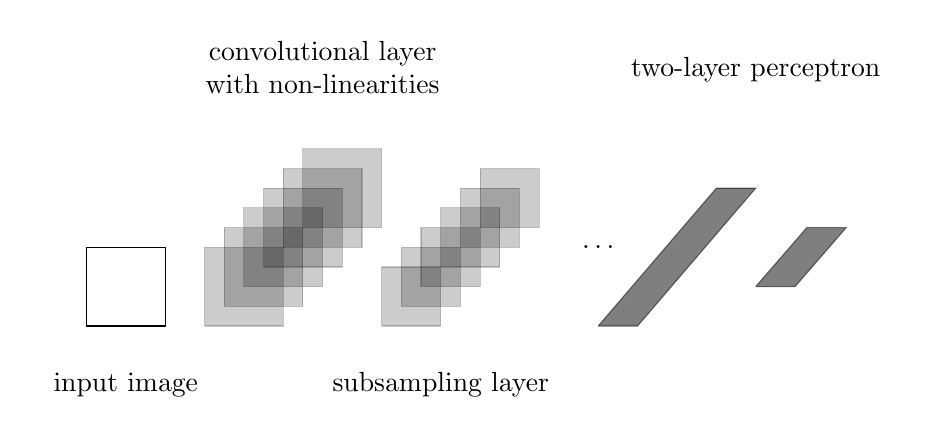
\begin{tikzpicture}

				\node at (0.5,-0.75){\begin{tabular}{c}input 
image\end{tabular}};
		
				\draw (0,0) -- (1,0) -- (1,1) -- (0,1) -- (0,0);
		
				\node at 
(3,3.25){\begin{tabular}{c}convolutional layer\\with 
non-linearities\end{tabular}};
		
				\draw[fill=black,opacity=0.2,draw=black] 
(2.75,1.25) -- (3.75,1.25) -- (3.75,2.25) -- (2.75,2.25) -- (2.75,1.25);
				\draw[fill=black,opacity=0.2,draw=black] 
(2.5,1) 
-- (3.5,1) -- (3.5,2) -- (2.5,2) -- (2.5,1);
				\draw[fill=black,opacity=0.2,draw=black] 
(2.25,0.75) -- (3.25,0.75) -- (3.25,1.75) -- (2.25,1.75) -- (2.25,0.75);
				\draw[fill=black,opacity=0.2,draw=black] 
(2,0.5) 
-- (3,0.5) -- (3,1.5) -- (2,1.5) -- (2,0.5);
				\draw[fill=black,opacity=0.2,draw=black] 
(1.75,0.25) -- (2.75,0.25) -- (2.75,1.25) -- (1.75,1.25) -- (1.75,0.25);
				\draw[fill=black,opacity=0.2,draw=black] 
(1.5,0) 
-- (2.5,0) -- (2.5,1) -- (1.5,1) -- (1.5,0);
		
				\node at 
(4.5,-0.75){\begin{tabular}{c}subsampling layer\end{tabular}};
		
				\draw[fill=black,opacity=0.2,draw=black] 
(5,1.25) -- (5.75,1.25) -- (5.75,2) -- (5,2) -- (5,1.25);
				\draw[fill=black,opacity=0.2,draw=black] 
(4.75,1) -- (5.5,1) -- (5.5,1.75) -- (4.75,1.75) -- (4.75,1);
				\draw[fill=black,opacity=0.2,draw=black] 
(4.5,0.75) -- (5.25,0.75) -- (5.25,1.5) -- (4.5,1.5) -- (4.5,0.75);
				\draw[fill=black,opacity=0.2,draw=black] 
(4.25,0.5) -- (5,0.5) -- (5,1.25) -- (4.25,1.25) -- (4.25,0.5);
				\draw[fill=black,opacity=0.2,draw=black] 
(4,0.25) -- (4.75,0.25) -- (4.75,1) -- (4,1) -- (4,0.25);
				\draw[fill=black,opacity=0.2,draw=black] 
(3.75,0) -- (4.5,0) -- (4.5,0.75) -- (3.75,0.75) -- (3.75,0);
		
% %				\node at 
% (7,3.5){\begin{tabular}{c}convolutional 
% layer\\with non-linearities\\layer $l = 4$\end{tabular}};
% %		
% %				\draw[fill=black,opacity=0.2,draw=black] 
% (7.5,1.75) -- (8.25,1.75) -- (8.25,2.5) -- (7.5,2.5) -- (7.5,1.75);
% %				\draw[fill=black,opacity=0.2,draw=black] 
% (7.25,1.5) -- (8,1.5) -- (8,2.25) -- (7.25,2.25) -- (7.25,1.5);
% %				\draw[fill=black,opacity=0.2,draw=black] 
% (7,1.25) -- (7.75,1.25) -- (7.75,2) -- (7,2) -- (7,1.25);
% %				\draw[fill=black,opacity=0.2,draw=black] 
% (6.75,1) -- (7.5,1) -- (7.5,1.75) -- (6.75,1.75) -- (6.75,1);
% %				\draw[fill=black,opacity=0.2,draw=black] 
% (6.5,0.75) -- (7.25,0.75) -- (7.25,1.5) -- (6.5,1.5) -- (6.5,0.75);
% %				\draw[fill=black,opacity=0.2,draw=black] 
% (6.25,0.5) -- (7,0.5) -- (7,1.25) -- (6.25,1.25) -- (6.25,0.5);
% %				\draw[fill=black,opacity=0.2,draw=black] 
% (6,0.25) -- (6.75,0.25) -- (6.75,1) -- (6,1) -- (6,0.25);
% %				\draw[fill=black,opacity=0.2,draw=black] 
% (5.75,0) -- (6.5,0) -- (6.5,0.75) -- (5.75,0.75) -- (5.75,0);
% %		
% %				\node at (9.5,-1){\begin{tabular}{c}subsampling 
% layer\\layer $l = 6$\end{tabular}};
% 		
% %				\draw[fill=black,opacity=0.2,draw=black] 
% (10,1.75) -- (10.5,1.75) -- (10.5,2.25) -- (10,2.25) -- (10,1.75);
% %				\draw[fill=black,opacity=0.2,draw=black] 
% (9.75,1.5) -- (10.25,1.5) -- (10.25,2) -- (9.75,2) -- (9.75,1.5);
% %				\draw[fill=black,opacity=0.2,draw=black] 
% (9.5,1.25) -- (10,1.25) -- (10,1.75) -- (9.5,1.75) -- (9.5,1.25);
% %				\draw[fill=black,opacity=0.2,draw=black] 
% (9.25,1) -- (9.75,1) -- (9.75,1.5) -- (9.25,1.5) -- (9.25,1);
% %				\draw[fill=black,opacity=0.2,draw=black] 
% (9,0.75) -- (9.5,0.75) -- (9.5,1.25) -- (9,1.25) -- (9,0.75);
% %				\draw[fill=black,opacity=0.2,draw=black] 
% (8.75,0.5) -- (9.25,0.5) -- (9.25,1) -- (8.75,1) -- (8.75,0.5);
% %				\draw[fill=black,opacity=0.2,draw=black] 
% (8.5,0.25) -- (9,0.25) -- (9,0.75) -- (8.5,0.75) -- (8.5,0.25);
% %				\draw[fill=black,opacity=0.2,draw=black] 
% (8.25,0) -- (8.75,0) -- (8.75,0.5) -- (8.25,0.5) -- (8.25,0);
% 		
				\node at (6.5,1){$\ldots$};
		
				\node at (8.5,3.25){\begin{tabular}{c}two-layer 
perceptron\end{tabular}};
		
				\draw[fill=black,draw=black,opacity=0.5] 
(6.5,0) 
-- (7,0) -- (8.5,1.75) -- (8,1.75) -- (6.5,0);
		
% 				%\node at (9,-1){\begin{tabular}{c}fully 
% connected layer\\output layer $l = 8$\end{tabular}};
		
				\draw[fill=black,draw=black,opacity=0.5] 
(8.5,0.5) -- (9,0.5) -- (9.65,1.25) -- (9.15,1.25) -- (8.5,0.5);
\end{tikzpicture}
\caption{A typical Convolutional Neural Network architecture}			
\end{figure}		
		
Convolutional Neural Networks have brought about a revolution in computer 
vision and is now the most successful approach for almost all recognition and 
detection tasks in computer vision 
\cite{krizhevsky2012imagenet,tompson2014efficient,taigman2014deepface} 
and some even approach human performance on some tasks 
\cite{ciresan2012multi}.\\

\subsubsection{Utilizing CNN's representation power}
\label{subsection:representation-discussion-cnn}
In~\ref{subsection:mistakes-learn}, we looked at a heuristic based game playing 
system called 
HOYLE~\cite{epstein-01_learning-to-play-expertly-tutorial-on-hoyle} that 
recorded a set of ``significant'' and ``dangerous'' states by exhaustively 
searching the tree, starting from states to look for alternate paths to win, 
whenever a game is lost. It is easy to understand that this system is not 
scalable to learning from a large set of games and neither can the applicability 
be explained with a small number of recorded states. However, the 
representation power of the convolutional neural networks can help in the 
representation of these ``dangerous'' and ``significant'' states. For instance, 
the first fully connected layer represents a n-dimensional space in which the 
similar states are embedded closer. This can significantly contribute to the 
HOYLE's strategy by providing a better generalization and efficient 
representation to the recorded states.

%XXX Describe this work in greater detail.

% \subsubsection{Playing Arcade Games using Convolutional Neural Networks}
% \label{subsubsection:deepmind}
% A remarkable work that helped bridge the gap between perception and action has 
% been Deepmind's deep reinforcement learning agent that is capable of learning 
% human-level control from high dimensional sensory input of an Atari video game 
% \cite{deepmind_nips}.\\
% 
% We tried to explore the last fully connected layer of a 
% convolutional neural network trained to play Breakout. The 
% figure~\ref{figure:deepmind} shows the apparent separation between the state 
% embeddings which are mapped to different actions.\\
% 
% \begin{figure}[h]
%  \centering
%  \hspace*{-1.2in}
%  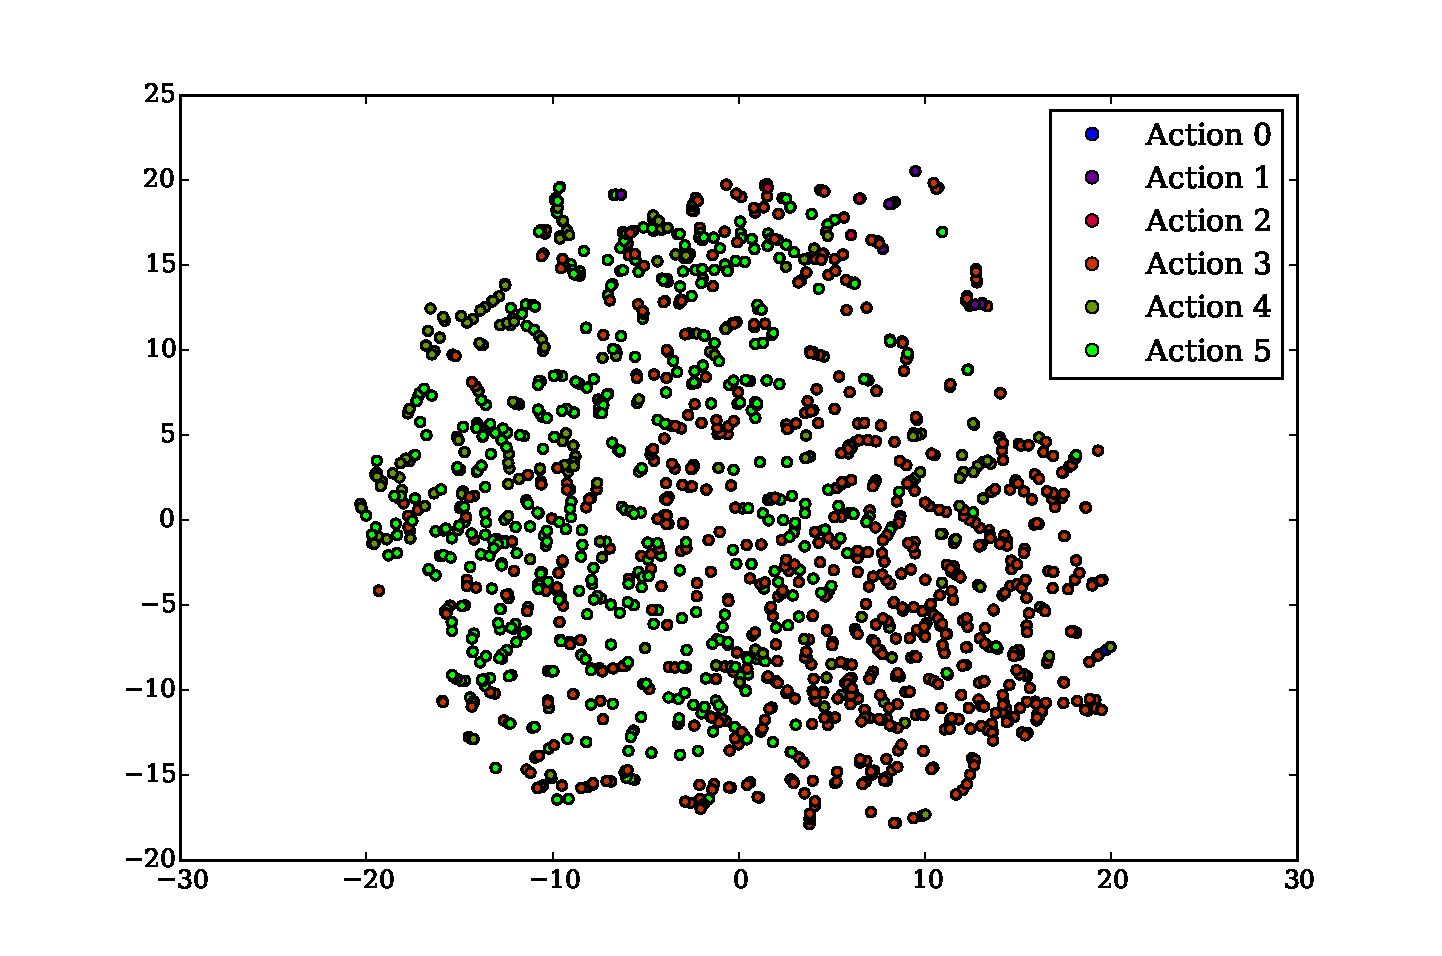
\includegraphics[width=1.5\textwidth]{plots/tsne_breakout_new.pdf}
%  
%  \caption[Fully connected layer's TSNE embedding in Deepmind's network]{The 
% plot shows the TSNE embedding of the last fully connected layer in a network 
% trained for the game of Breakout. The two primary colors--green and brown, 
% respectively, show the two primary actions learned while playing the game of 
% Breakout i.e. left and right respectively and the separation is almost 
% apparent. }
% \label{figure:deepmind}
% \end{figure}
% 
% 
% An extension of this work by \citet*{guo2014deep} 
% improved the results a bit on some games that required extensive planning. They 
% used a Monte-Carlo tree search based player to simulate trajectories, before 
% using the generated state-action-value instances to train a CNN based 
% regression model. The method proved to make a fruitful integration of a 
% planning agent and the RL agent in a way similar to the one discussed 
% in section~\ref{section:RL}.\\ 
% 
% Along with the TSNE embedding in figure~\ref{figure:deepmind}, builds our 
% intuition that the subspace that the convolutional neural network embeds the 
% state representations (i.e. the game screens) in Breakout on the basis of the 
% most favorable action for that state. We will see that 
% regardless of the task specification i.e. either we choose Q-learning (e.g. in 
% \citet{deepmind_nips}) or we choose a regression or classification task (e.g. 
% in \citet{guo2014deep}), we are almost asking the network to embed the states 
% effectively to select the best action.\\
% 
% This is the major motivation to our method of learning the evaluation 
% function for chess boards (state) based on the final outcome of the games, 
% which we describe in the next chapter.

\section*{Organization of the thesis}
The thesis is organized in the classic style of first introducing the problem 
and discussing related work (chapter~\ref{chap:introduction}), 
then chapter~\ref{chap:implementation} where we describe 
our dataset representation and implementation details while 
systematically moving towards our aim. Finally we present the results and 
analysis (chapter~\ref{chap:results}). In the chapter~\ref{chap:implementation}, 
we specifically mention the convolutional neural network architecture we use, 
the loss functions and the how we employ them to choose a move while playing a 
game of chess. In the results chapter, we describe the strengths and weaknesses 
of our system by considering specific case studies. Finally, we conclude with a 
discussion about the feasibility of such systems and how they can be a part of 
the future of computer chess.